
\begin{figure}[bh!]
\centering
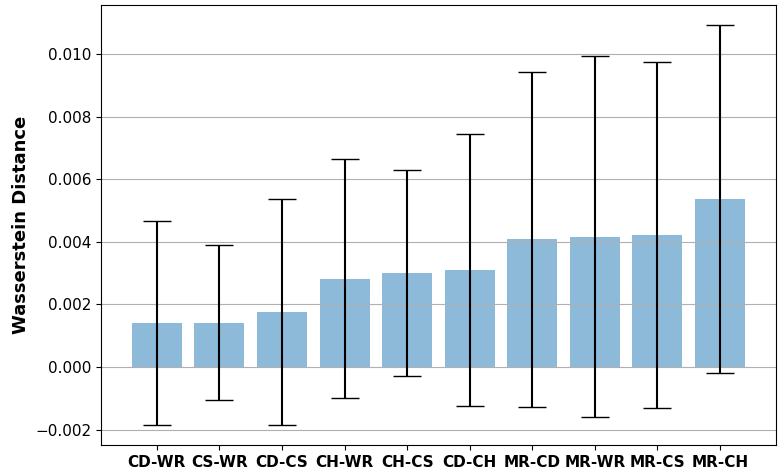
\includegraphics[width=1\columnwidth]{Figures/ErrorBarComparisons2Cultivars.png} % Reduce the figure size so that it is slightly narrower than the column. Don't use precise values for figure width.This setup will avoid overfull boxes.
\caption{Error bars of pairwise cultivar comparisons. The mean of each comparison is the height of the bars while the standard deviation is the height of the error bars.}
\label{fig:paircultivar}
\end{figure}


\begin{figure}[th!]
\centering
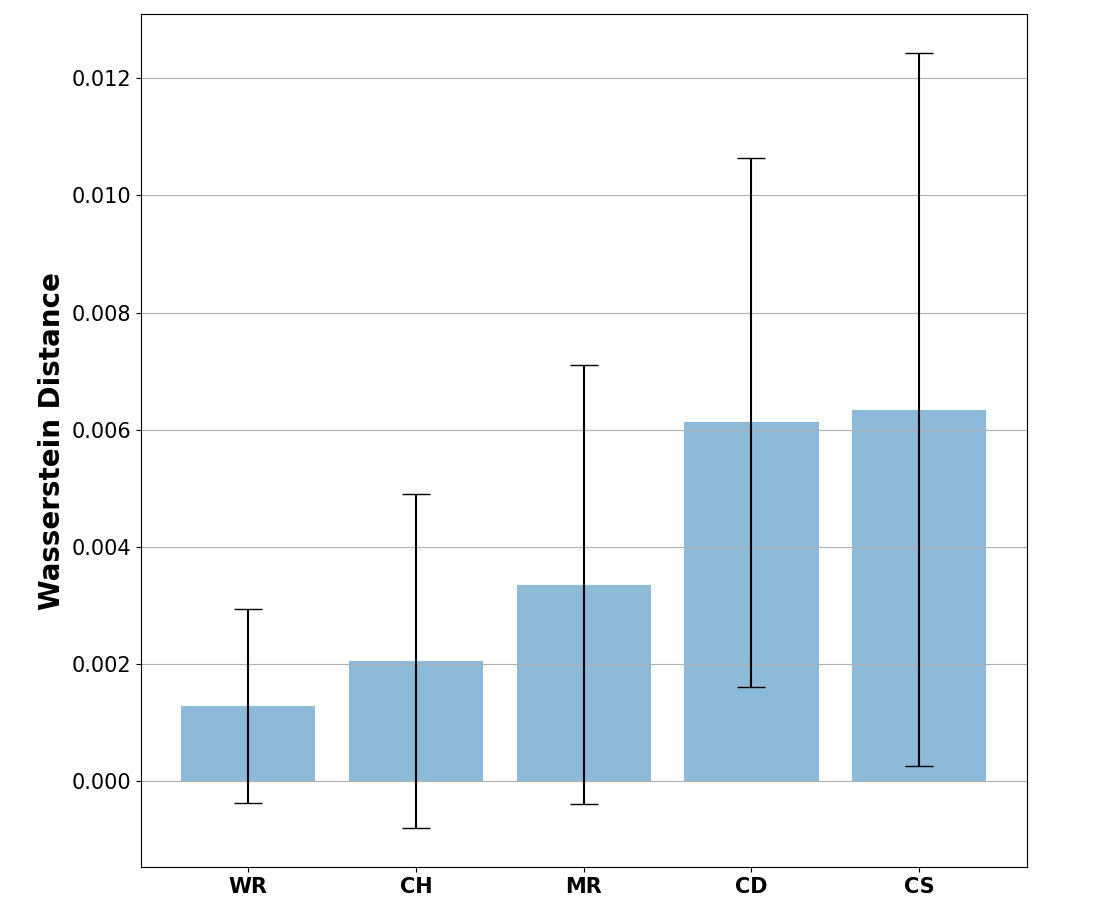
\includegraphics[width=1\columnwidth]{Figures/ErrorBarComparisons10seasons.png} % Reduce the figure size so that it is slightly narrower than the column. Don't use precise values for figure width.This setup will avoid overfull boxes.
\caption{Error bars of pairwise seasons comparisons for each cultivar.}
\label{fig:pairseason}
\end{figure}






\subsection{Seasonal comparisons}
\label{sec:results:seasonalcompare}
Table~\ref{tab:distance_matrix_seasons} shows the distance matrix for comparing the last 5 seasons, using the methodology described in Task 2 of Section~\ref{sec:PDforCH}.
The following observations can be made. 
a) The distance values range within a tight interval of [0.070, 0.101], with an average of 0.088. 
b) The largest distance was observed between the season pairs 2017-2018 vs. 2019-2020, while the smallest was for 2017-2018 vs. 2021-2022. 
c) On average though, the season 2018-2019 showed the maximum distance from all other seasons. 
This can be easily confirmed by visually inspecting the persistence diagrams shown for all 5 seasons in Figure~\ref{fig:PDpairseasons}.


In addition to the last five years, we compared all pairs of seasons (results not shown due to space limit). We observed that the two most different seasons (i.e., with the largest Wasserstein distance) were the seasons 2001-2002 vs. 2010-2011 (shown 
in Figure~\ref{fig:holesseason}). 


\begin{table}[htp]
\centering
\resizebox{1\columnwidth}{!}{
\begin{tabular}{ |l|r|r|r|r|r|}
\hline
&	\multicolumn{1}{|c|}{\textbf{2017-2018}}	&	\multicolumn{1}{|c|}{\textbf{2018-2019}}	&	\multicolumn{1}{|c|}{\textbf{2019-2020}}	&	\multicolumn{1}{|c|}{\textbf{2020-2021}}	&	\multicolumn{1}{|c|}{\textbf{2021-2022}}\\\hline
\textbf{2017-2018}	&	0	&	0.099	&	\emph{0.101}	&	0.089	&	\emph{0.070}\\\hline
\textbf{2018-2019}	&	0.099	&	0	&	0.086	&	0.086	&	0.092\\\hline
\textbf{2019-2020}	&	0.101	&	0.086	&	0	&	0.085	&	0.087\\\hline
\textbf{2020-2021}	&	0.089	&	0.086	&	0.085	&	0	&	0.089\\\hline
\textbf{2021-2022}	&	0.070	&	0.092	&	0.087	&	0.089	&	0\\\hline
\end{tabular}
}
\caption{Pairwise distance matrix for selected seasons (2017 to 2022). Each value shows the Wasserstein distance between the $\mathrm{dgm}_1$ obtained for the corresponding two seasons.
}
\label{tab:distance_matrix_seasons}
\end{table}